\documentclass[11pt,t,usepdftitle=false,aspectratio=169]{beamer}
\usepackage{biblatex}
\usepackage{color}

\definecolor{green}{RGB}{0,220,0}
\definecolor{orange}{RGB}{240,200,0}
\definecolor{blue}{RGB}{0,0,255}

\addbibresource{bibliography.bib}

\usetheme[nototalframenumber,foot,logo]{uibk}

%% information for the title page
\title[Erkennung von Resampling]{Erkennung von Resampling}
\subtitle{InterpoLIE-tion - Catching lies through interpolation analysis}

\author[Dominik Barbist, Lukas Egger]{Dominik Barbist, Lukas Egger \\ \vspace{0.5em}}
\footertext{Digitale Forensik mit Bild- und Videodaten}
\date{\today}

\headerimage{3}

\begin{document}

%% this sets the first PDF bookmark and triggers generation of the title page
\section{Introduction}

\begin{frame}
	\frametitle{Übersicht}
	
	\textbf{Struktur der Präsentation:}
	
	\vspace{1.5em}
	
	\begin{enumerate}
		\setlength{\itemsep}{0.8em}
		\item \textbf{Einführung} - Was ist Resampling?
		\item \textbf{Kartoffel-Contest} - Praktisches Beispiel
		\item \textbf{Grundprinzip} - Warum detektierbar?
		\item \textbf{Detektions-Methoden} - Algorithmische Ansätze
		\item \textbf{Zusammenfassung} - Forensik in der Praxis
	\end{enumerate}
\end{frame}

\subsection{Einführung}

\begin{frame}
	\frametitle{Das unsichtbare Verbrechen: Digitale Bildmanipulation}
	
	\begin{columns}[T]
		\begin{column}{0.48\textwidth}
			\begin{exampleblock}{Das perfekte Verbrechen?}
				\begin{itemize}
					\item \textbf{Kinderleicht} - skalieren, drehen, strecken
					\item \textbf{Unsichtbar} - keine sichtbaren Spuren (wenn gut gemacht)
				\end{itemize}
			\end{exampleblock}
		\end{column}
		\begin{column}{0.48\textwidth}
			\textbf{Die Lösung:}
			\begin{itemize}
				\item \textcolor{blue}{Interpolation} hinterlässt mathematische Spuren
				\item \textcolor{blue}{Algorithmen} können diese detektieren
				\item \textcolor{blue}{Automatische} Forensik möglich
			\end{itemize}
		\end{column}
	\end{columns}
	
	\vspace{0.5em}
	
	\begin{alertblock}{Das Problem}
		Jeder kann zum \textcolor{red}{Fälscher} werden! (... bei genügend Übung)
	\end{alertblock}
	
	\begin{block}{Die Herausforderung}
		Computer sehen, was Menschen übersehen.
	\end{block}
\end{frame}

\subsection{Kartoffel-Contest Szenario}

\begin{frame}
	\frametitle{Welche Kartoffel ist gefälscht?}
	\begin{columns}[T]
		\begin{column}{0.48\textwidth}
			\centering
			\textbf{Kartoffel A}
			\vspace{0.5em}
			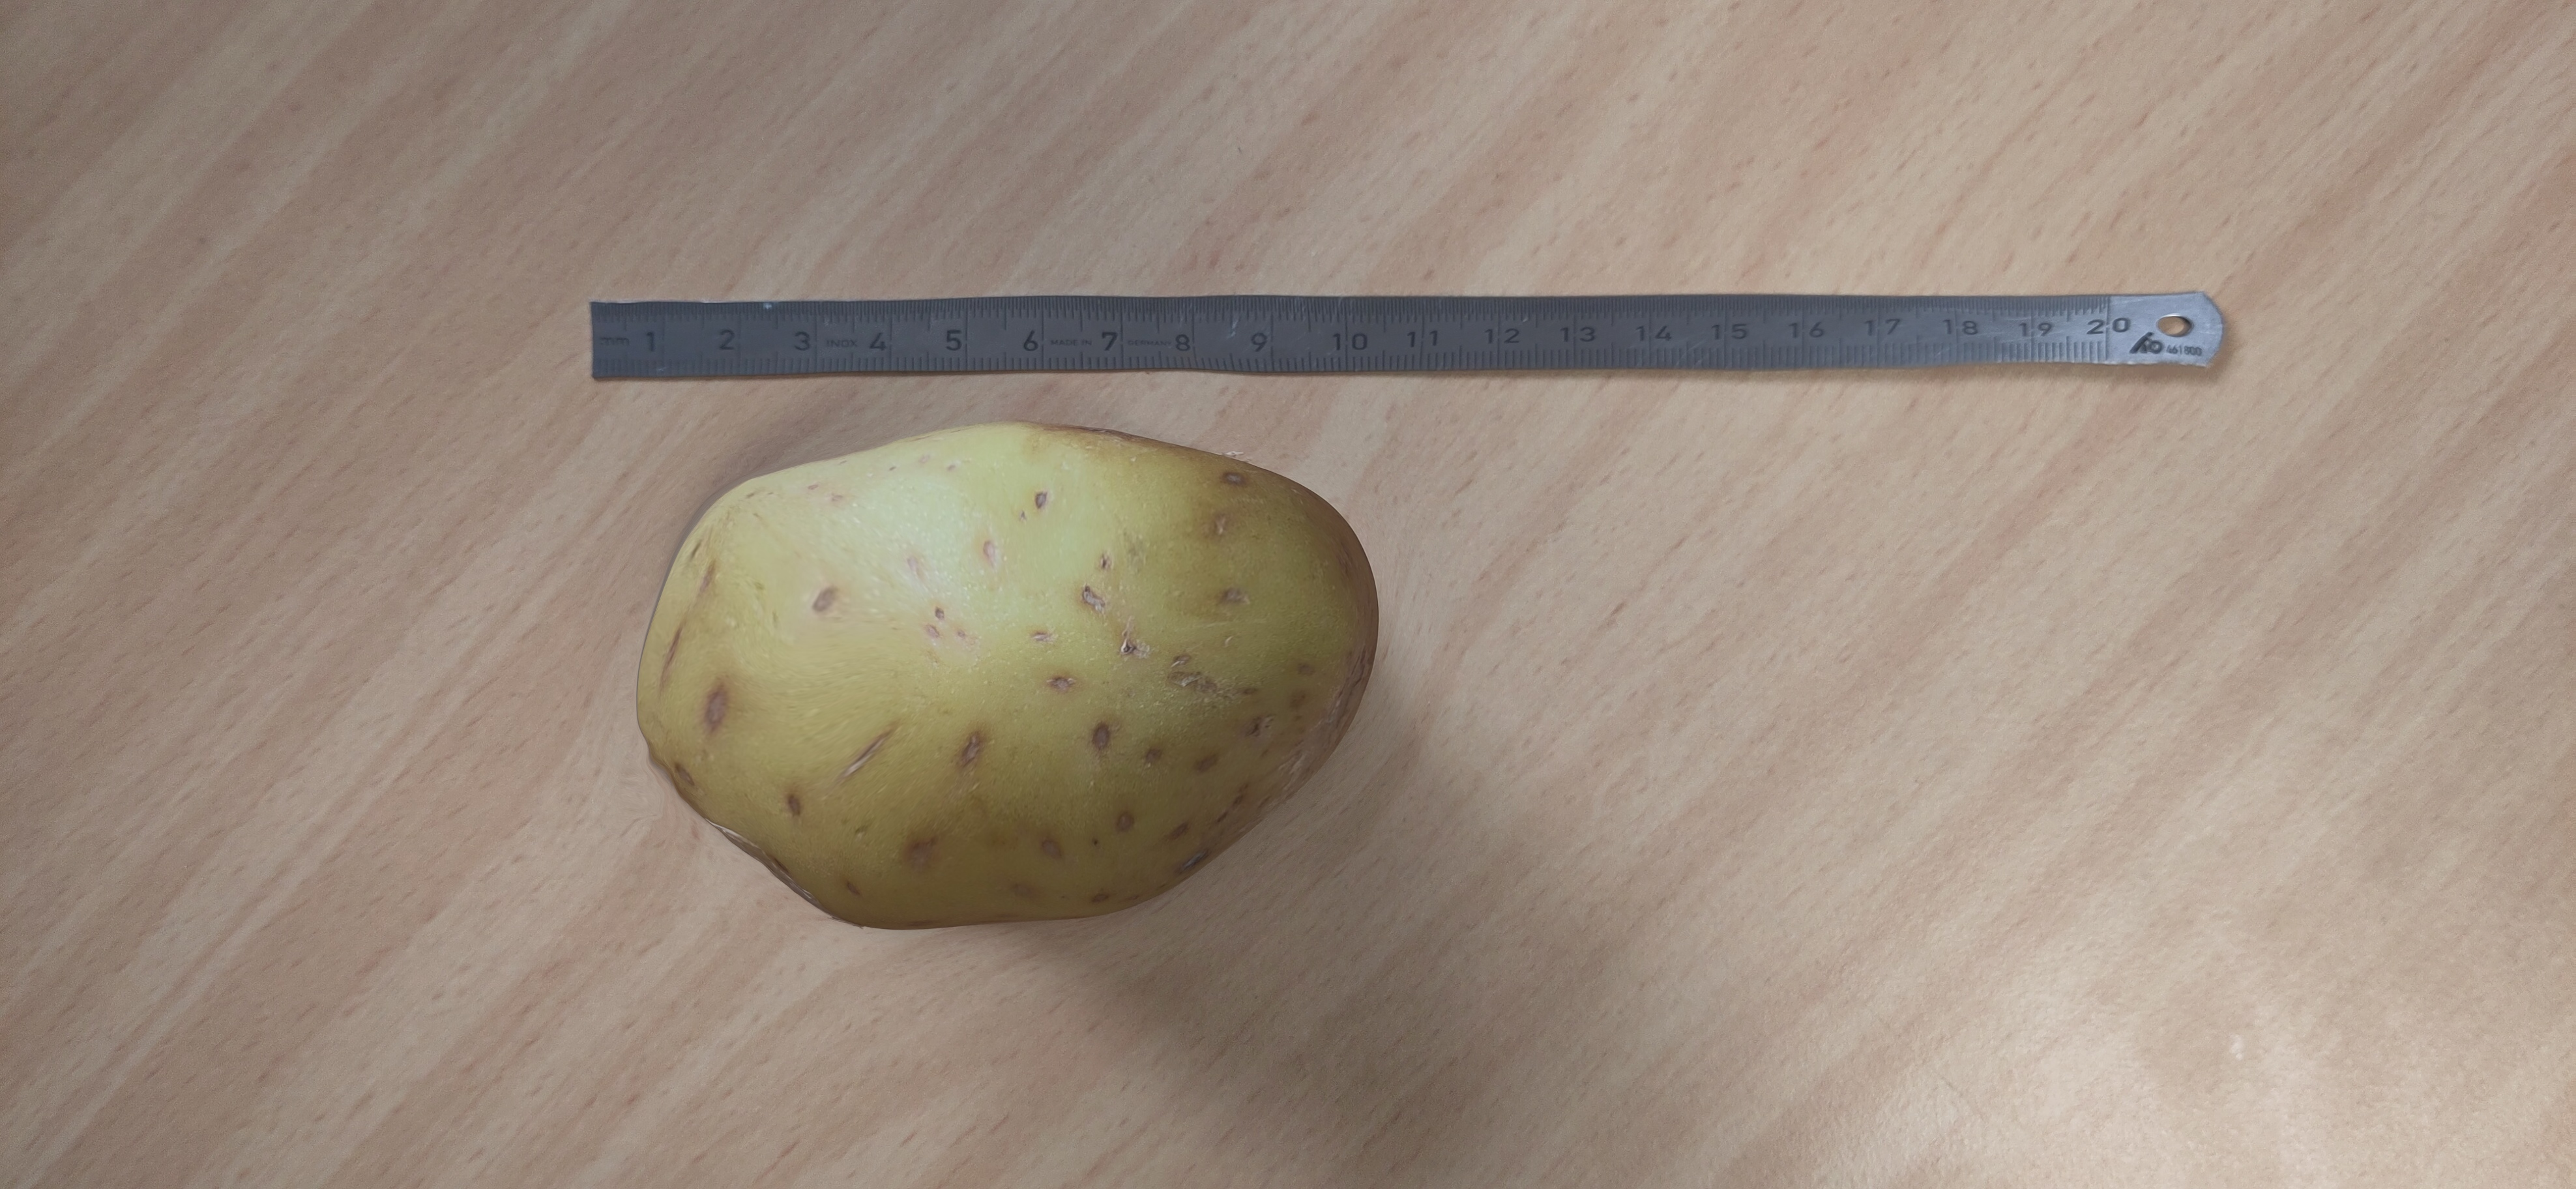
\includegraphics[width=\textwidth]{images/image_2_s.jpg}
		\end{column}
		\begin{column}{0.48\textwidth}
			\centering
			\textbf{Kartoffel B}
			\vspace{0.5em}
			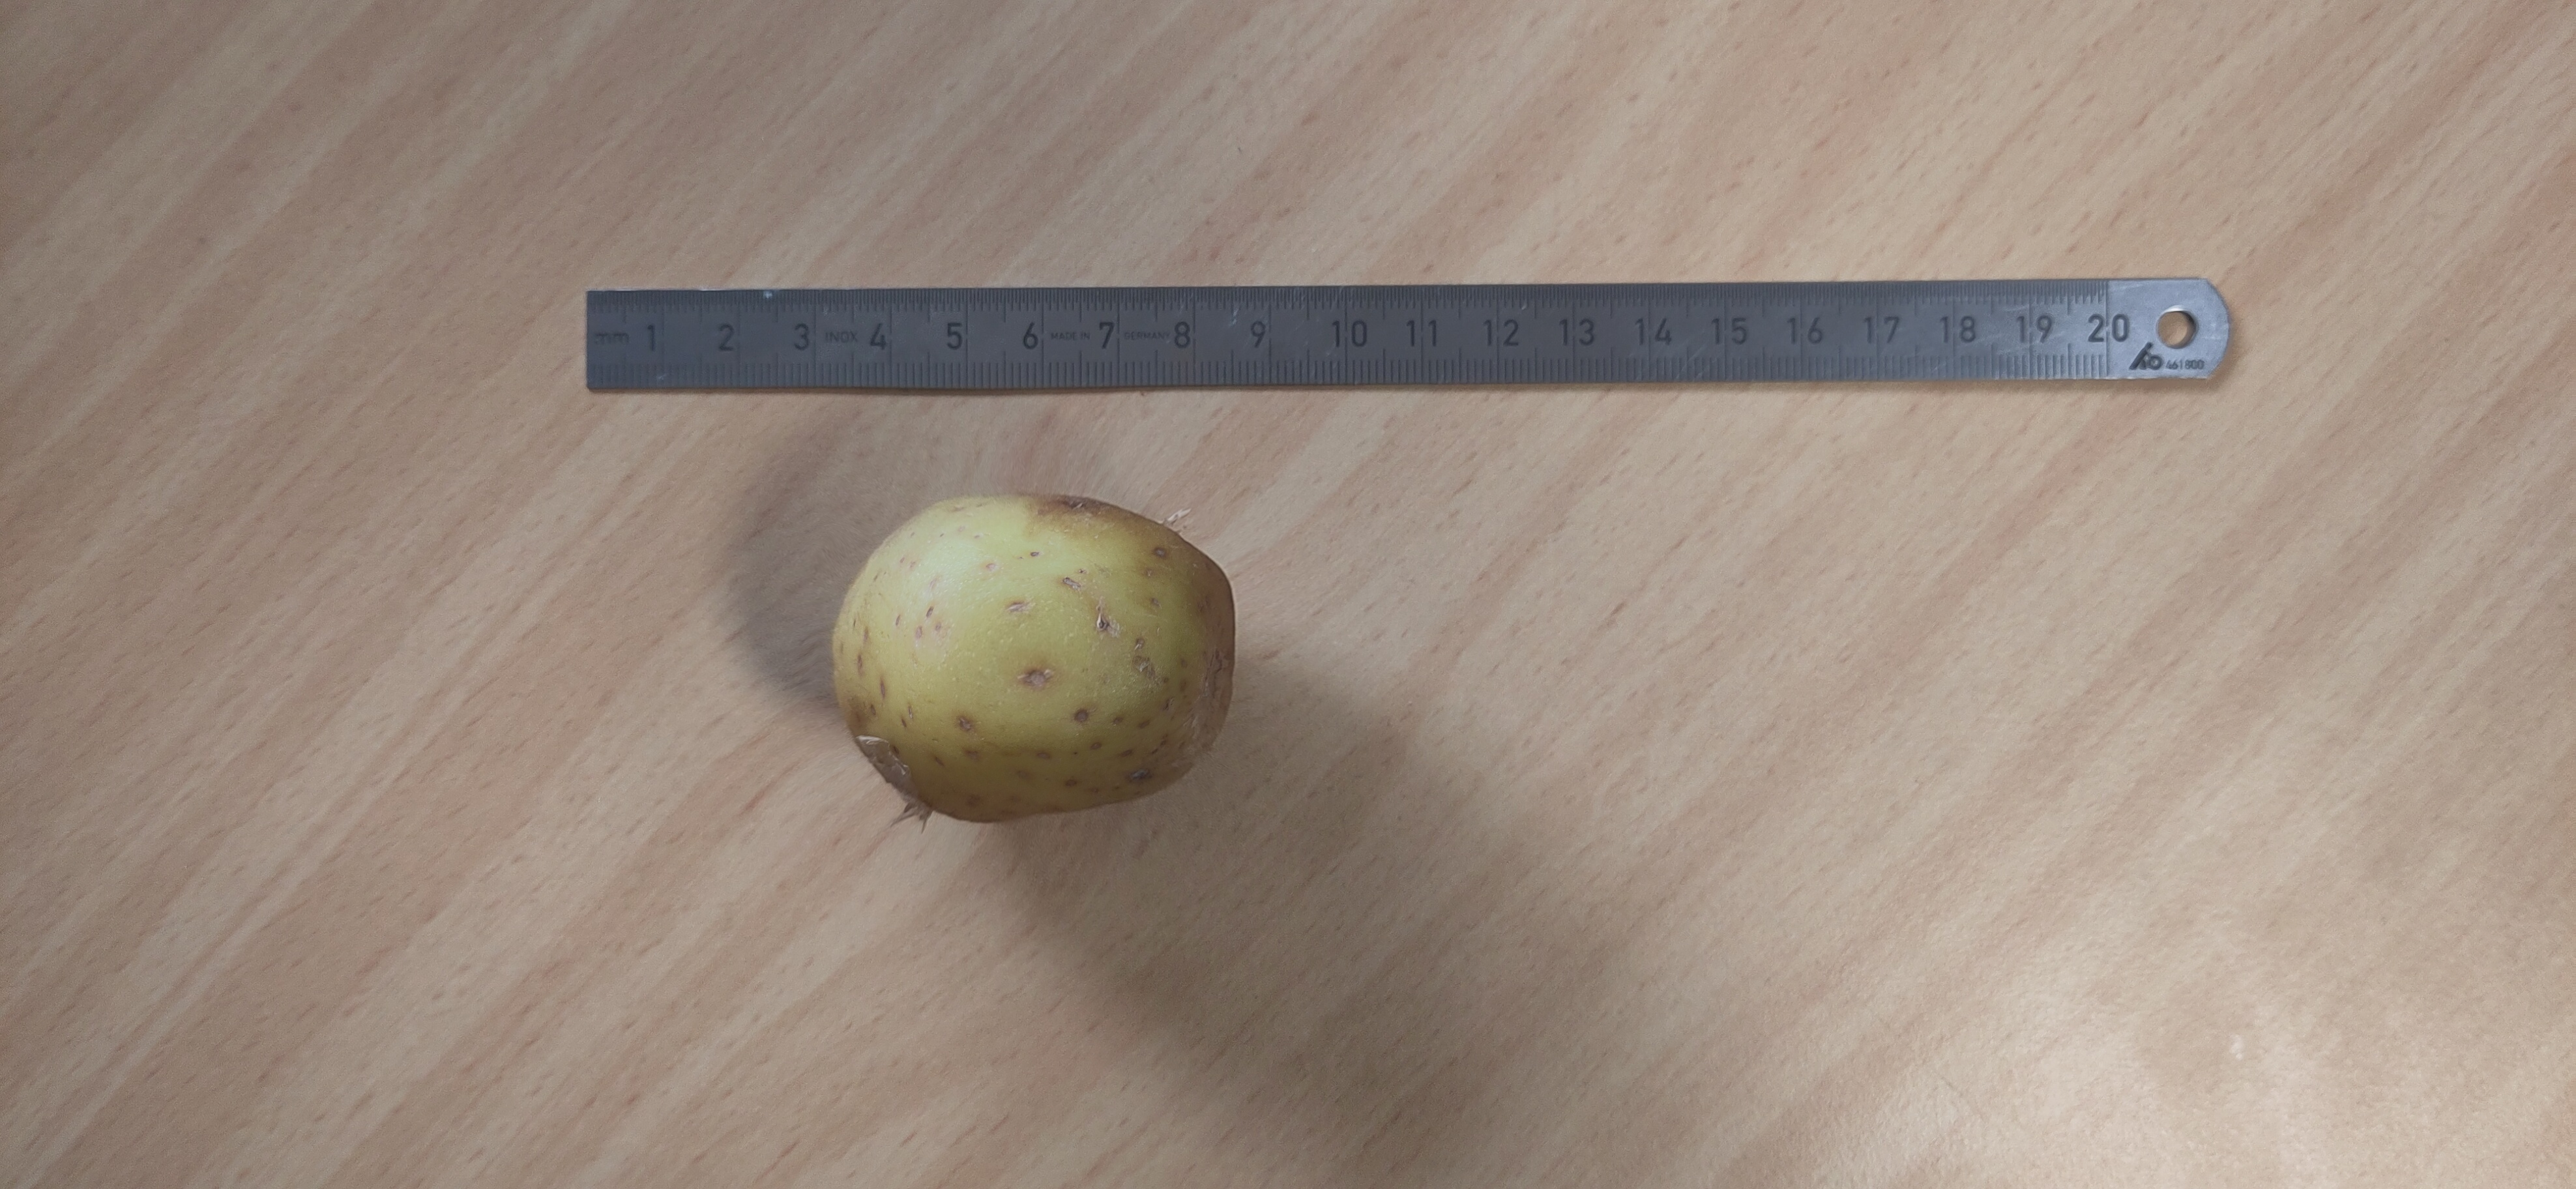
\includegraphics[width=\textwidth]{images/image_2_s2.jpg}
		\end{column}
	\end{columns}
	
	\vspace{2em}
	\begin{alertblock}{Frage}
		Welche Kartoffel wurde digital manipuliert? A oder B?
	\end{alertblock}
\end{frame}

\begin{frame}
	\frametitle{Überraschung: Beide waren gefälscht!}
	\begin{columns}[T]
		\begin{column}{0.48\textwidth}
			\textbf{Die Wahrheit:}
			\begin{itemize}
				\item \textcolor{red}{Beide Bilder} waren manipuliert
				\item Das \textcolor{green}{echte Original} sieht anders aus
				\item Manipulation war \textcolor{orange}{nicht unmittelbar erkennbar}
			\end{itemize}
			
			\vspace{0.5em}
			\textbf{Das Problem:}
			\begin{itemize}
				\item Visuelle Inspektion \textcolor{red}{reicht nicht}
				\item Professionelle Manipulation \textcolor{red}{täuscht}
				\item Automatische Detektion \textcolor{blue}{erforderlich}
			\end{itemize}
		\end{column}
		\begin{column}{0.48\textwidth}
			\centering
			\textbf{Das echte Original:}
			\vspace{0.5em}
			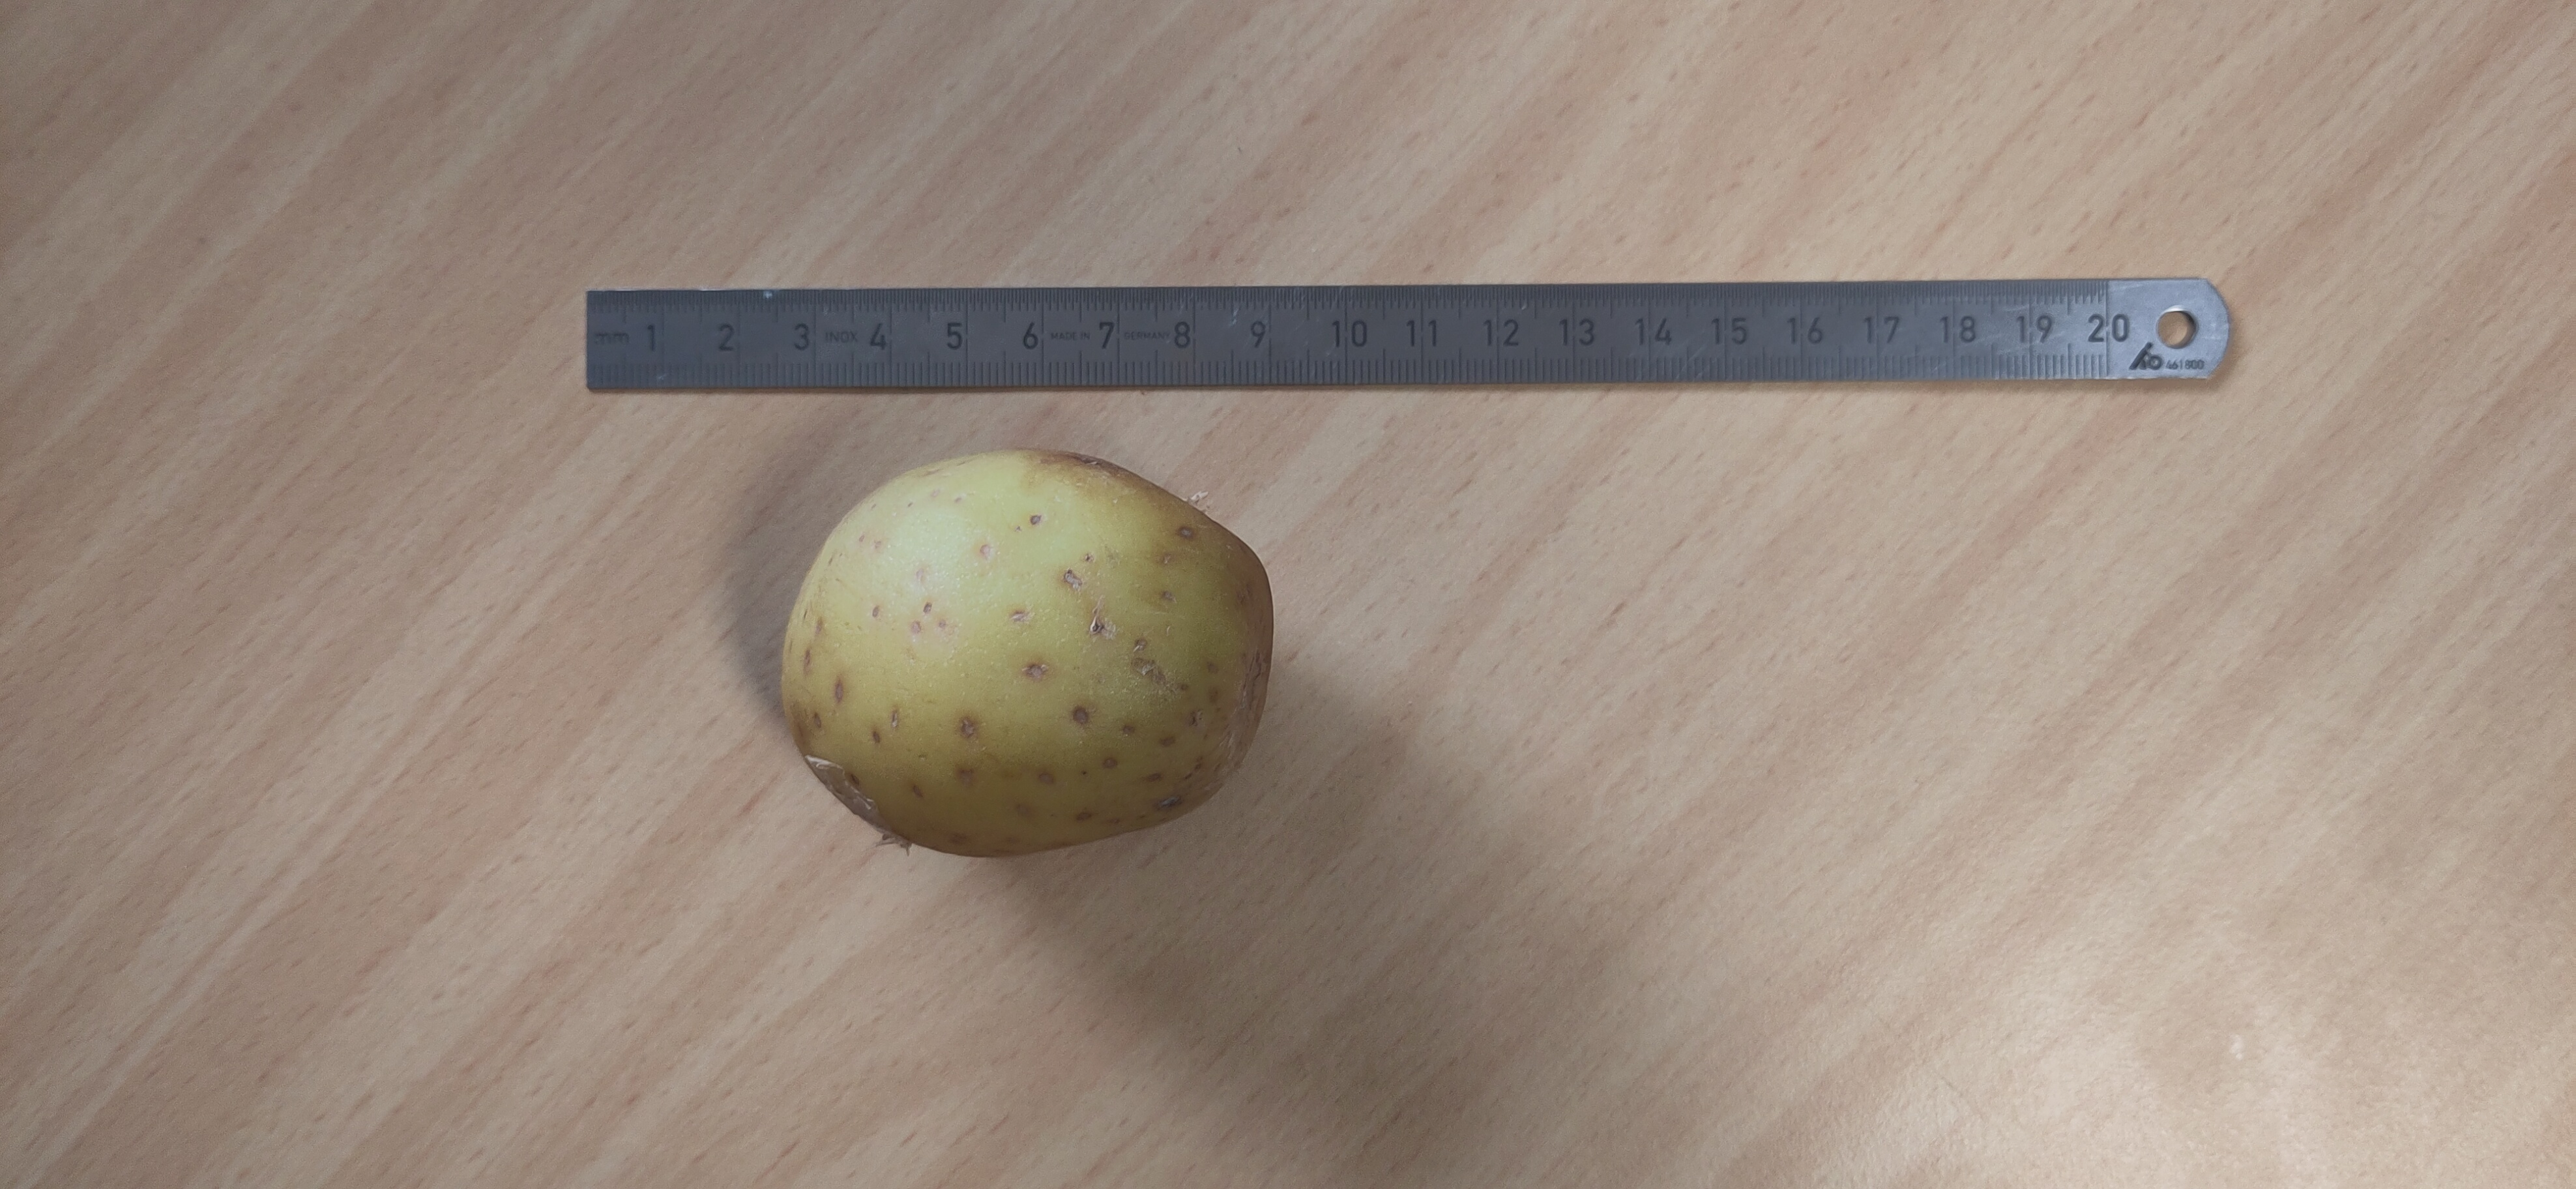
\includegraphics[width=\textwidth]{images/image_2.jpg}
			\vspace{0.5em}
			\textcolor{green}{\textbf{Unmanipuliert}}
		\end{column}
	\end{columns}
\end{frame}

\begin{frame}
	\frametitle{Kartoffel-Contest: Das Szenario}
	\begin{columns}[T]
		\begin{column}{0.48\textwidth}
			\textbf{Online-Größenwettbewerb:}
			\begin{itemize}
				\item Teilnehmer fotografieren \textcolor{blue}{größte Kartoffeln}
				\item \textcolor{blue}{Maßband/Lineal} als Größenreferenz
				\item Upload auf Contest-Plattform
				\item Gewinner erhält Preisgeld
			\end{itemize}
		\end{column}
		\begin{column}{0.48\textwidth}
			\textbf{Die Herausforderung:}
			\begin{itemize}
				\item Betrug durch \textcolor{red}{Resampling}
				\item Kartoffel vergrößern, Maßband verkleinern
				\item Proportionen \textcolor{orange}{bleiben stimmig}
				\item Manipulation \textcolor{orange}{unsichtbar}
			\end{itemize}
		\end{column}
	\end{columns}
	
	\vspace{1.5em}
	\begin{alertblock}{Die Lösung}
		\textbf{Resampling Detection} kann solche Manipulationen automatisch aufdecken.
	\end{alertblock}
\end{frame}


\subsection{Lösungsansätze}

\begin{frame}
	\frametitle{Das Problem: Was passiert beim Skalieren?}
	\begin{columns}[T]
		\begin{column}{0.48\textwidth}
			\textbf{Was passiert beim Skalieren:}
			\begin{enumerate}
				\item \textbf{Neue Pixel-Positionen} berechnen
				\item \textbf{Interpolation:} Fehlende Werte schätzen
				\item \textbf{Lineare Abhängigkeiten} entstehen
			\end{enumerate}
		\end{column}
		\begin{column}{0.48\textwidth}
			\textbf{Beispiel - Kartoffel 2x vergrößern:}
			\begin{itemize}
				\item Original: 100x100 Pixel
				\item Skaliert: 200x200 Pixel  
				\item \textcolor{red}{Problem:} 30.000 neue Pixel müssen "erfunden" werden
			\end{itemize}
		\end{column}
	\end{columns}
	
	\vspace{1.5em}
	\begin{alertblock}{Das Problem}
		Interpolation erzeugt \textbf{mathematische Regelmäßigkeiten} statt natürlicher Zufälligkeit.
	\end{alertblock}
\end{frame}

\begin{frame}
	\frametitle{Die Lösung: Resampling-Spuren detektieren}
	\begin{columns}[T]
		\begin{column}{0.48\textwidth}
			\textbf{Interpolation hinterlässt Spuren:}
			\begin{itemize}
				\item \textcolor{blue}{Periodische Muster} in Pixelwerten
				\item \textcolor{blue}{Statistische Korrelationen} zwischen Nachbarn
				\item \textcolor{blue}{Frequenz-Peaks} in der Spektralanalyse
			\end{itemize}
		\end{column}
		\begin{column}{0.48\textwidth}
			\textbf{Detektions-Strategie:}
			\begin{itemize}
				\item Suche nach \textbf{unnatürlichen Mustern}
				\item Analysiere \textbf{Pixel-Abhängigkeiten}
				\item Erkenne \textbf{mathematische Periodizität}
			\end{itemize}
		\end{column}
	\end{columns}
	
	\vspace{1.5em}
	\begin{alertblock}{Kernidee}
		Echte Fotos haben \textbf{zufällige} Pixelwerte, interpolierte Bilder zeigen \textbf{mathematische Regelmäßigkeiten}.
	\end{alertblock}
\end{frame}

\begin{frame}
	\frametitle{Lösungsansätze: Wie kann man Resampling detektieren?}
	\begin{itemize}
		\item \textbf{Popescu \& Farid (2005)~\cite{popescu_exposing_2005}:} EM-Algorithmus → Wahrscheinlichkeitskarte
		\item \textbf{Kirchner (2008)~\cite{kirchner_fast_2008}:} Feste Filter → Spektralanalyse  
		\item \textbf{Gallagher (2005)~\cite{gallagher_detection_2005}:} JPEG-Blöcke → Varianz-Periodizität
		\item \textbf{Mahdian \& Saic (2008)~\cite{mahdian_blind_2008}:} Radon-Transform → Rotations-robust
		\item \textbf{Feng et al. (2012)~\cite{noauthor_pdf_2024}:} Energie-Dichte → Machine Learning
		\item \textbf{Vázquez-Padín (2015)~\cite{vazquez-padin_svd_2015}:} SVD-Analyse → Kleine Bildblöcke
	\end{itemize}
	
	\vspace{1.5em}
	\begin{alertblock}{Gemeinsamer Ansatz}
		Alle Methoden suchen nach \textbf{mathematischen Mustern}, die durch Interpolation entstehen.
	\end{alertblock}
\end{frame}

\subsection{Zusammenfassung}

\begin{frame}
	\frametitle{Zusammenfassung: Kartoffel-Contest und digitale Forensik}
	\begin{columns}[T]
		\begin{column}{0.48\textwidth}
			\textbf{Das Problem:}
			\begin{itemize}
				\item Skalierungs-Betrug schwer erkennbar
				\item Proportionen sehen korrekt aus
				\item Visuelle Inspektion reicht nicht
			\end{itemize}
			
			\vspace{1em}
			\textbf{Die Lösung:}
			\begin{itemize}
				\item Interpolation hinterlässt Spuren
				\item Mathematische Detektion möglich
				\item Automatisierte Forensik-Analyse
			\end{itemize}
		\end{column}
		\begin{column}{0.48\textwidth}
			\textbf{Herausforderungen:}
			\begin{itemize}
				\item JPEG-Kompression
				\item Kleine Skalierungsfaktoren
				\item Geschwindigkeit vs. Genauigkeit
			\end{itemize}
		\end{column}
	\end{columns}
\end{frame}

\subsection{Quellen}
\begin{frame}
    \frametitle{Quellen}
    \begingroup
    \setbeamerfont{bibliography item}{size=\tiny}
    \setbeamerfont{bibliography entry author}{size=\tiny}
    \setbeamerfont{bibliography entry title}{size=\tiny}
    \setbeamerfont{bibliography entry location}{size=\tiny}
    \setbeamerfont{bibliography entry note}{size=\tiny}
    \setbeamerfont{bibliography entry year}{size=\tiny}
    \setlength{\bibitemsep}{2pt}
    \setlength{\itemsep}{0pt}
    \setlength{\parskip}{0pt}
    \renewcommand{\bibfont}{\tiny}
    \printbibliography[heading=none]
    \endgroup
\end{frame}

%% to show a last slide similar to the title slide
\title[Erkennung von Resampling]{Erkennung von Resampling}
\subtitle{InterpoLIE-tion - Catching lies through interpolation analysis}
\section{Vielen für Ihre Aufmerksamkeit!}


\end{document}